\section{Test Case Setup}\label{intro}
This part will set up a mimetic spectral element solver for a scalar Laplace equation. The theoretical description will not be elaborated here but the implementation detail will be recorded to serve the major purpose of this report. \\

\subsection{Scalar Laplace Equation (Poisson Equation)}
The Scalar Laplace equation is given in \ref{scalarlaplace}:
\begin{subequations}\label{scalarlaplace} 
	\begin{align}
		-\Delta \phi(x,y) &= f, \ \ (x,y) \in \Omega \\
		BC: \phi(x,y) &= \phi_{tr}, \ \ (x,y) \in \partial \Omega.
	\end{align}

\end{subequations}
To apply mimetic spectral element method to discretise this equation, equation is re-written in the following system of partial differential equations. The new system has equation \ref{gradphi} and \ref{divq}, two purely topological equations, and one extra constitutive equation \ref{hodgetrans} that connects an $1$-form to an $(n-1)$-form. 
\begin{subequations}\label{eqnsystem}
	\begin{align} \label{gradphi}
		\vect{d}\phi^{(0)} &= \vect{u^{(1)}}, \\ \label{hodgetrans}
		\star \vect{u^{(1)}} &= \vect{\tilde{q}^{(n-1)}}, \\ \label{divq}
		\vect{d}\vect{\tilde{q}^{(n-1)}} &= f^{(n)}.
	\end{align}
\end{subequations}
The equation system can be deliberately used for discretisation. \\

\subsection{Discretisation of Poisson Equation}
This part will discretise the equation system \ref{eqnsystem} one by one, and then construct the discretised linear equation system.\\

Before writing all the equations out with variables, we place a Tonti Graph at the top first. Then referring to the graph, we can make certain rules for the notions of basis and variables. A Tonti diagram is given in figure \ref{Tontigraph}. We let variables with a hat $\hat{\ }$ denote their own basis function, and if we remove the notions' subscription in the Tonti diagram, they will represent the degrees of freedom on cochain. \\
\begin{figure}[H]
\centering
	\begin{tikzpicture}
		\matrix (m) [matrix of math nodes, row sep=3em, column sep=4em,minimum width=2em]
  {
     \phi^{(0)} & \vect{u^{(1)}} \\
     f^{(n)} & \vect{\tilde{q}^{(n-1)}} \\};
  \path[-stealth]
    (m-1-1) edge[<->] node [right] {$\star$} (m-2-1)
            edge[->] node [above] {$\vect{d}$} (m-1-2)
    (m-2-1) edge[<-] node [above] {$\vect{d}$} (m-2-2)
    (m-1-2) edge[<->] node [right] {$\star$} (m-2-2);
\end{tikzpicture}
\caption{Tonti Diagram}
\label{Tontigraph}
\end{figure}


\subsubsection{Gradient Equation: $\vect{d} \phi^{(0)} = \vect{u^{(1)}}$}
On the left-hand-side of the gradient equation, $\phi^{(0)}$ is a scalar function defined on calculation domain $\Omega$. It admits a projection $\Pi_h$ that projects itself to a finite dimensional space $Q =span\{h_i(x) \otimes h_j(y)\},\ i,j = 0,1,2,...,n $: 
\begin{equation}
	\Pi_h(\phi^{(0)}) = \phi_{(i,j)} \cdot \left(h_i^{(0)}(x) \otimes h_j^{(0)}(y) \right) = \phi_{k(i,j)} \cdot \hat{\phi}^{(0)}_{k(i,j)}\ .
\end{equation}
After projection, function $\phi$ is expanded by the nodal basis functions $\hat{\phi}^{(0)}_{k}$, where $k(i,j)$ is a compression mapping that maps a 2D location array into 1D. This compression mapping affects the shape and sparsity pattern of the coefficient matrix of the final equation system. \\

Similarly, on the right-hand-side, the vector $\vect{u^{(1)}}$ admits another expansion given by:
\begin{align}
	\Pi_h(\vect{u^{(1)}}) &= u_{(i,j)} \cdot \left(\vect{e_i^{(1)}}(x) \otimes h_j^{(0)}(y) \right) + v_{(j,i)} \cdot \left(h_i^{(0)}(x) \otimes \vect{e_j^{(1)}}(y) \right) \\
	 &= u_{K(i,j)} \cdot \hat{u}_{K(i,j)}^{(1)}\ ,
\end{align}
where $K(i,j)$ is the compression mapping that controls the sequence of the degrees of freedom. According to the construction of the edge function, $d(\alpha^{(0)})=\sum_{i=0}^{N}(\alpha_i \cdot h_i(x) ) = \sum_{i=1}^{N}(\alpha_i - \alpha_{i-1})\cdot\vect{e_i^{(1)}} $. Then the gradient equation will be:
\begin{equation}
	\left[\vect{E_{K\times k}^{(1,0)}}\right] \cdot \phi _{k(i,j)} = \vect{u}_{K(i,j)}\ .
\end{equation} 

\subsubsection{Divergence Equation: $\vect{d\tilde{q}^{(n-1)}} = -f^{(n)}$}
Similar to the previous gradient equation, we write the discretised system directly:
\begin{equation}
	\left[\vect{\tilde{E}_{k\times K}^{(n,n-1)}}\right] \cdot \vect{\tilde{q}}_{K(i,j)} = {f}_{k(i,j)}\ .
\end{equation}
In this relation, both $k$ and $K$ will take the same compression numbering scheme as the previous gradient equation. \\

\subsubsection{Constitutive Relation: $\star\vect{u^{(1)}} = \vect{\tilde{q}^{(n-1)}}$}
We use the $\vect{L^2}$ inner product of flux vector $\vect{\tilde{q}^{(n-1)}}$ and its basis function sets to measure the local metrics:
\begin{subequations}
\begin{align}
	\left<\vect{\tilde{q}^{(n-1)}},\ \vect{\hat{q}^{(n-1)}}  \right>_{\vect{L^2}, \Omega} &= \int_{\Omega} \left(\star\vect{\tilde{q}^{(n-1)}} \wedge \vect{\hat{q}^{(n-1)}}  \right) \\
	&= \int_{\Omega} \star\star \left(\vect{{u}^{(1)}} \wedge \vect{\hat{q}^{(n-1)}}  \right) \\
	&= (-1)^{n(n-k)}\cdot \int_{\Omega} \left(\vect{{u}^{(1)}} \wedge \vect{\hat{q}^{(n-1)}}  \right) \\
	&= \int_{\Omega} \left(\vect{d}\phi^{(0)} \wedge \vect{\hat{q}^{(n-1)}}  \right) \\
	&= \int_{\Omega} \vect{d}\left(\phi^{(0)} \cdot \vect{\hat{q}^{(n-1)}}  \right) - \int_{\Omega} \phi^{(0)} \vect{d\hat{q}^{(n-1)}}  . 
\end{align}
\end{subequations}
The left-hand-side gives a discrete system:
\begin{equation}
	\left<\vect{\tilde{q}^{(n-1)}},\ \vect{\hat{q}^{(n-1)}}  \right>_{\vect{L^2}, \Omega} = \left[\vect{M^{(n-1)}_{K\times K}} \right]\cdot \vect{q_{K(i,j)}}, 
\end{equation}
and the right-hand-side will be:
\begin{equation}
	\int_{\Omega} \vect{d}\left(\phi^{(0)} \cdot \vect{\hat{q}^{(n-1)}}  \right) - \int_{\Omega} \phi^{(0)} \vect{d\hat{q}^{(n-1)}} = \left[\vect{B^{(n-1,0)}} \right]\cdot \phi^{}_{tr} - \left[\vect{E^{(n,n-1)^T}_{k\times K}} \vect{W^{(n,0)}_{k\times k}}\right]\cdot \phi_{k(i,j)}. 
\end{equation}
Thus the discretised system will be: 
\begin{equation}
	\left[\vect{M^{(n-1)}_{K\times K}} \right]\cdot \vect{q_{K(i,j)}} + \left[\vect{E^{(n,n-1)^T}_{k\times K}} \vect{W^{(n,0)}_{k\times k}}\right]\cdot \phi_{k(i,j)} = \left[\vect{B^{(n-1,0)}} \right]\cdot \phi^{}_{tr} 
\end{equation}

\subsubsection{Final Discrete Equation System}
The final discretised linear equation system of a single spectral element is: 
\begin{equation}
	\begin{bmatrix}
		\vect{M^{(n-1)}_{K\times K}} &  \vect{E^{(n,n-1)^T}_{k\times K}} \vect{W^{(n,0)}_{k\times k}}\\
		\vect{W^{(n,0)^T}_{k\times k}}\vect{E_{k\times K}^{(n,n-1)}} & \vect{O} 
	\end{bmatrix}
	\begin{bmatrix}
		\vect{\tilde{q}}\\ \phi
	\end{bmatrix}
	=
	\begin{bmatrix}
		\vect{B^{(n-1,0)}}\phi^{}_{tr}\\
		\vect{W^{(n,0)^T}_{k\times k}}{f}_{k(i,j)}
	\end{bmatrix}.
\end{equation}
This is the starting point of the first preconditioning test case. \\

\section{Analysis of the Final System}
To analyse the condition of a saddle point linear equation system, we establish a common routine for such tasks. First of all, one will have to inspect the condition number of the mass matrix $\vect{M}$, incidence matrices $\vect{E}$, Schur complement of the mass matrix in the discrete system $\vect{S}$, and the wedge product matrix $\vect{W}$. In particular, one should find how the condition numbers scale with the problem size. The first step is done and the results are shown in table \ref{chartcond} and figure \ref{cond} below. In results, $\vect{LHS}$ is the full system's coefficient matrix, and $\vect{map}$ is defined by $\vect{map} = \vect{E_{k\times K}^{(n,n-1)}}\cdot \vect{E_{k\times K}^{(n,n-1)^T}}$. \\

\begin{table}[H]
	\centering
	\caption{Condition Number of Matrices}
	\label{chartcond}
	\begin{tabular}{|c|c|c|c|c|} 
		\hline
		p-order & 5& 9 & 13 & 25 \\ [0.5ex] \hline 
		$\vect{M^{(n-1)}}$ & 33.35 & 88.39 & 170.53 & 578.33 \\[0.5ex] \hline
		$\vect{S}$ & 29.90 & 106.39 & 248.40 & 1301.06 \\[0.5ex] \hline
		$\vect{LHS}$ &22.60 & 24.20 & 48.82 & 251.93 \\[0.5ex] \hline
		$\vect{map}$ & 13.93 & 39.86 & 78.77 & 273.31 \\[0.5ex]\hline
		$\vect{W^{(0,n)}}$ & 1.82 & 2.06 & 2.17 & 2.30 \\ 
		\hline
	\end{tabular}
\end{table}
The results show the same situation recorded in other similar literatures. The Schur complement matrix $\vect{S}$ has the worst condition, and $\kappa(\vect{M})$ also grows fast with the problem size. This is a "signature" symptom of many traditional PDE induced saddle point systems, where methods like Uzawa algorithm and Bramble-Pasciak CG become costly. \\
   
\begin{figure}[H]
	\centering
	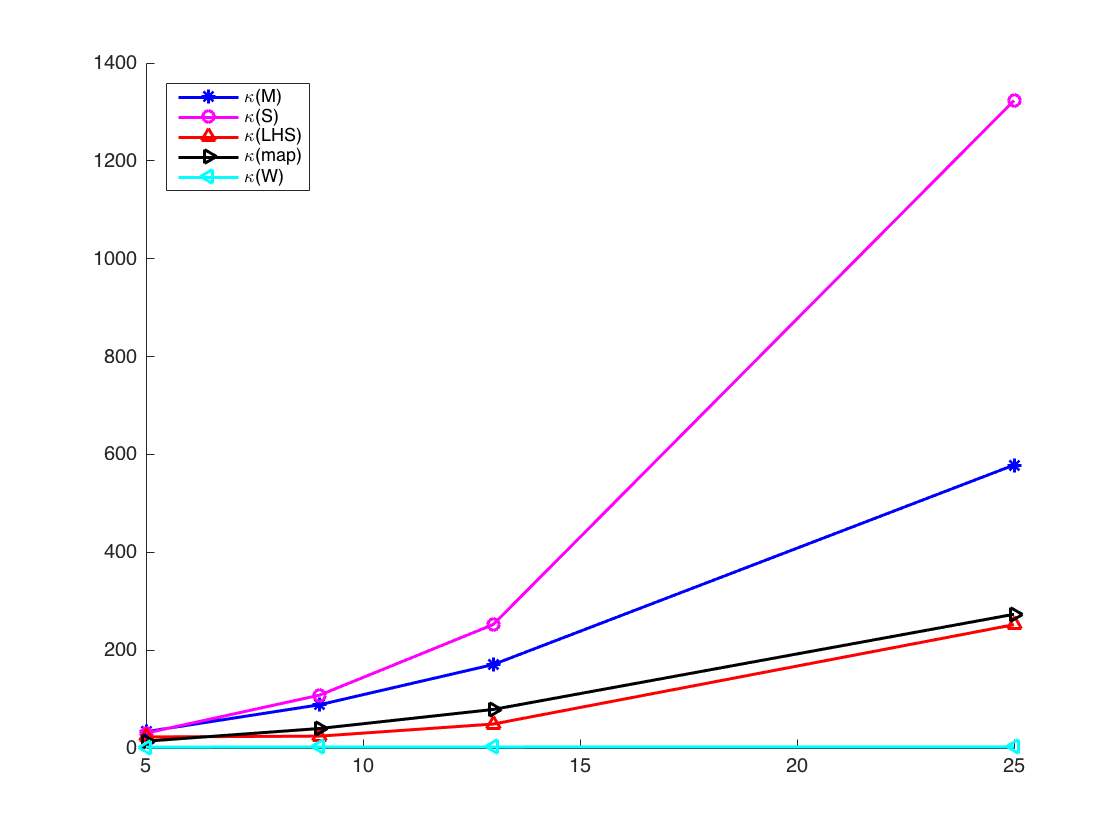
\includegraphics[width=.85\textwidth]{cond}
	\caption{Condition Number of the System}
	\label{cond}
\end{figure}
In the result, we could see that the wedge product matrix do not vary with the problem size, an intuitive explanation is that the wedge product in this case is a metric-free operation, thus unlike the mass matrix, it will not be affected by the mesh density. Another interesting observation is that the condition number of the full system and the condition number of the so called $\vect{map}$ matrix change synchronously. From the minimisation problem perspective, we are solving a scalar Laplace equation and $\vect{q}$ is an intermediate function that minimises the energy, thus the condition of the full system is determined by the Laplacian part. To further illustrate this idea, it's found that the condition of a properly scaled block diagonal matrix $\mathcal{A}$ in equation \ref{blkdiagcond} is bounded only by the $(2,2)$ block, which means that the "Laplacian" accounts for worsening the condition of the left-hand-side matrix.  
\begin{equation}\label{blkdiagcond}
	\kappa(\mathcal{A}) = \min_{\lambda>0} \left\lbrace \kappa
	\begin{pmatrix}
		\vect{\lambda M} & \vect{O} \\
		\vect{O} & \vect{W^T E M^{-1} E^T W} \\
	\end{pmatrix}	 \right\rbrace = \kappa\left(\vect{W^T E M^{-1} E^T W} \right) 
\end{equation}
This observation rings a bell of why constraint preconditioners are applied. About this phenomena, I give a short explanation of why I choose to inspect such a $\vect{map}$ matrix. This $\vect{map}$ matrix is exactly the finite difference 5-point Laplace operator. In the mimetic discretisation framework, this is equivalent to a finite difference discrete scalar Laplacian that applies on a uniform mesh. The coming work would have to work with the $\vect{map}$ matrix instead of the incidence matrix to reduce the Schur complement condition number.    \\

The first inspection tells us about the possibilities of the coming work. We may try the traditional block diagonal preconditioning techniques first. After that, we could also try constraint preconditioners. To achieve these goals, we first need a powerful mass matrix approximation. In addition, traditional approaches also requires an algorithm to calculate preconditioner for the Schur complement. The coming subsections will prepare these basic elements first.  \\

\subsection{Mass Matrix Approximation}
The mass matrix of a $(n-1)$-form is obtained by calculating the inner product of the set of $(n-1)$-form basis functions.
%\begin{equation}
%	\vect{M^{(n-1)}} = \left\langle \vect{\hat{q}^{n-1}_{K_1}} \ ,\ \vect{\hat{q}^{n-1}_{K_2}} \right\rangle _{\vect{L^2,\ \Omega}}. 
%\end{equation}
Each mass matrix element $m_{(K_1,K_2)}$ is calculated by: 
\begin{equation}
	m_{(K_1,K_2)} = \left\langle \vect{\hat{q}^{n-1}_{K_1(p,q)}} \ ,\ \vect{\hat{q}^{n-1}_{K_2(m,n)}} \right\rangle _{\vect{L^2,\ \Omega}} .
\end{equation}
Since $\vect{\hat{q}^{n-1}_{K}}$ is a compressed array with both $\vect{u}$ and $\vect{v}$ basis, if they are stored in the 1D array as two separated subarrays like $[\vect{u_{basis}}...,\vect{v_{basis}}...]$, the mass matrix will be a 2-by-2 block diagonal matrix. Further more, since the $\vect{u_{basis}}$ and $\vect{v_{basis}}$ inherited the symmetry from the co-ordinate system in a quadrilateral mesh, the mass matrix will have a repeating diagonal block if the compression mapping $K$ is "symmetrical" applied on both vector basis. This idea is shown in figure \ref{symm_basis}.\\
 
\begin{figure}[H]
	\centering
	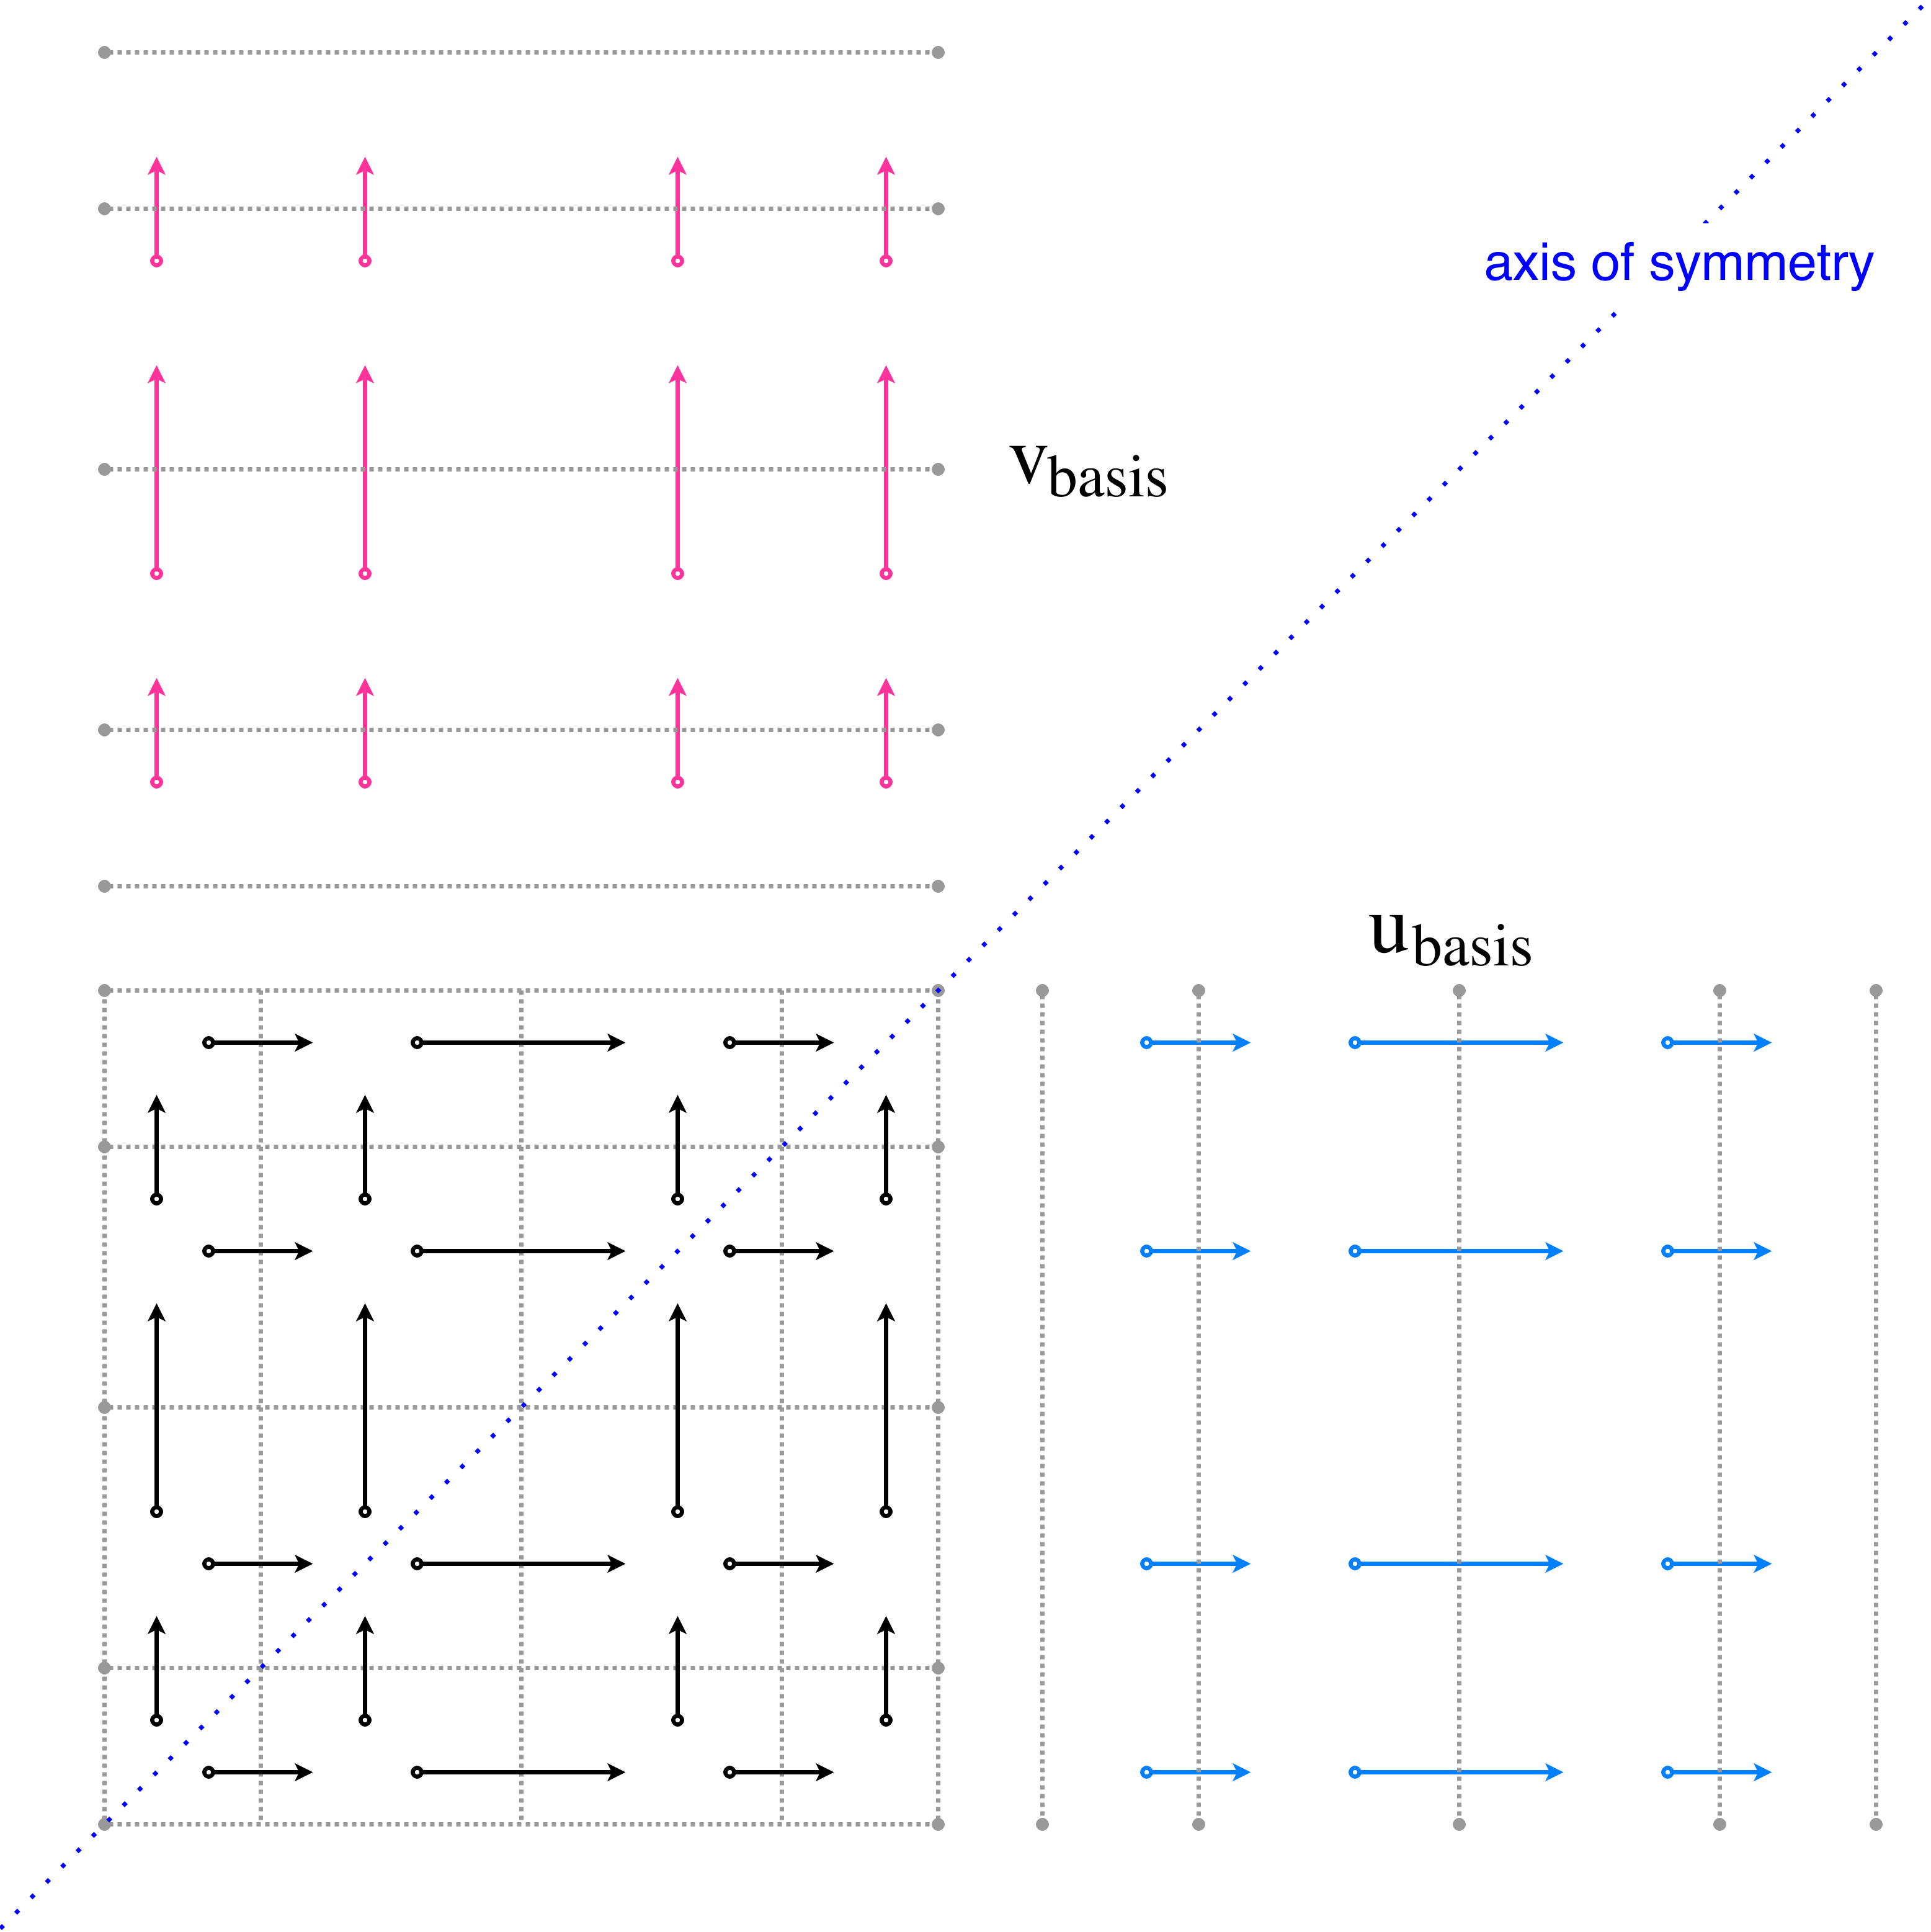
\includegraphics[width=.85\textwidth]{basis_symmetry}
	\caption{Symmetry of Vectors}
	\label{symm_basis}
\end{figure}  
Based on the previous analysis, I computed a mass matrix with polynomial expansion degree $p=5$, using a standard GLL mesh. The mass matrix surface plot and sparsity pattern are shown in figure \ref{mass_surf} and \ref{mass_spy}.\\
\begin{figure}[H]
	\minipage{0.45\textwidth}
	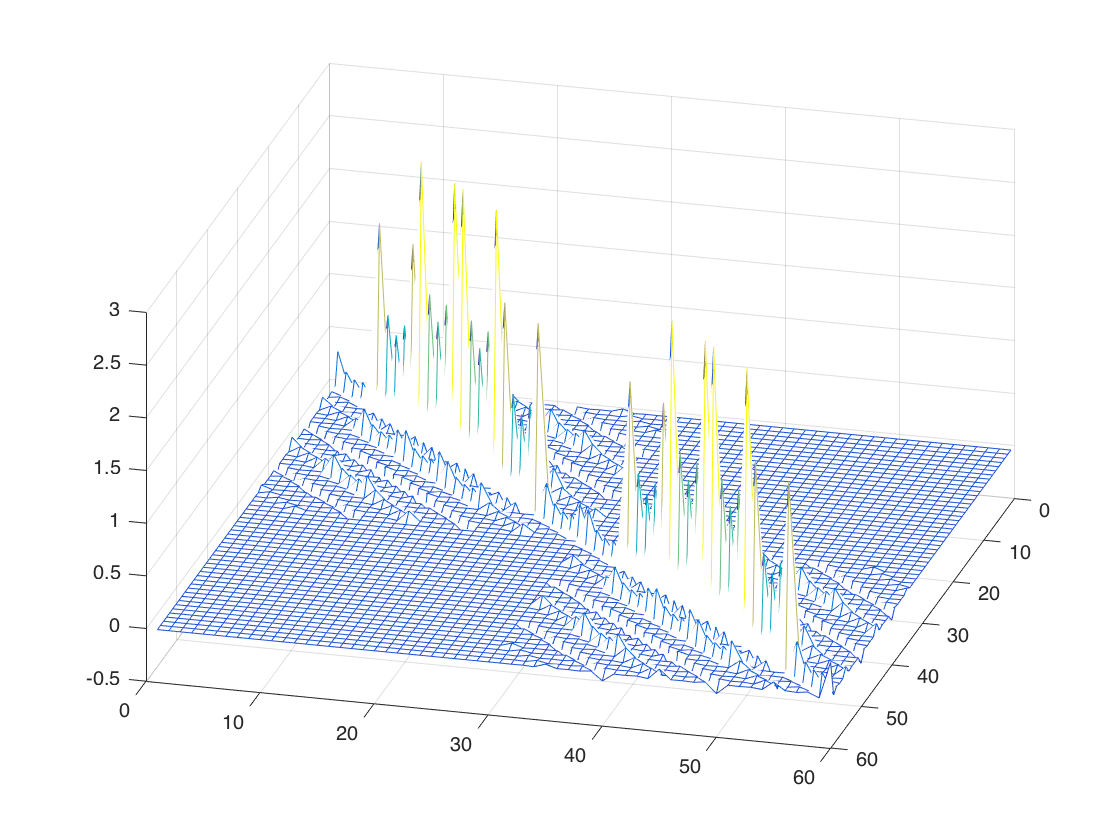
\includegraphics[width=\linewidth]{full_mass_quad_2p}
	\caption{$\vect{M^{(n-1)}}$ with $p=5$}
	\label{mass_surf}
	\endminipage \hfill
	\minipage{0.45\textwidth}
	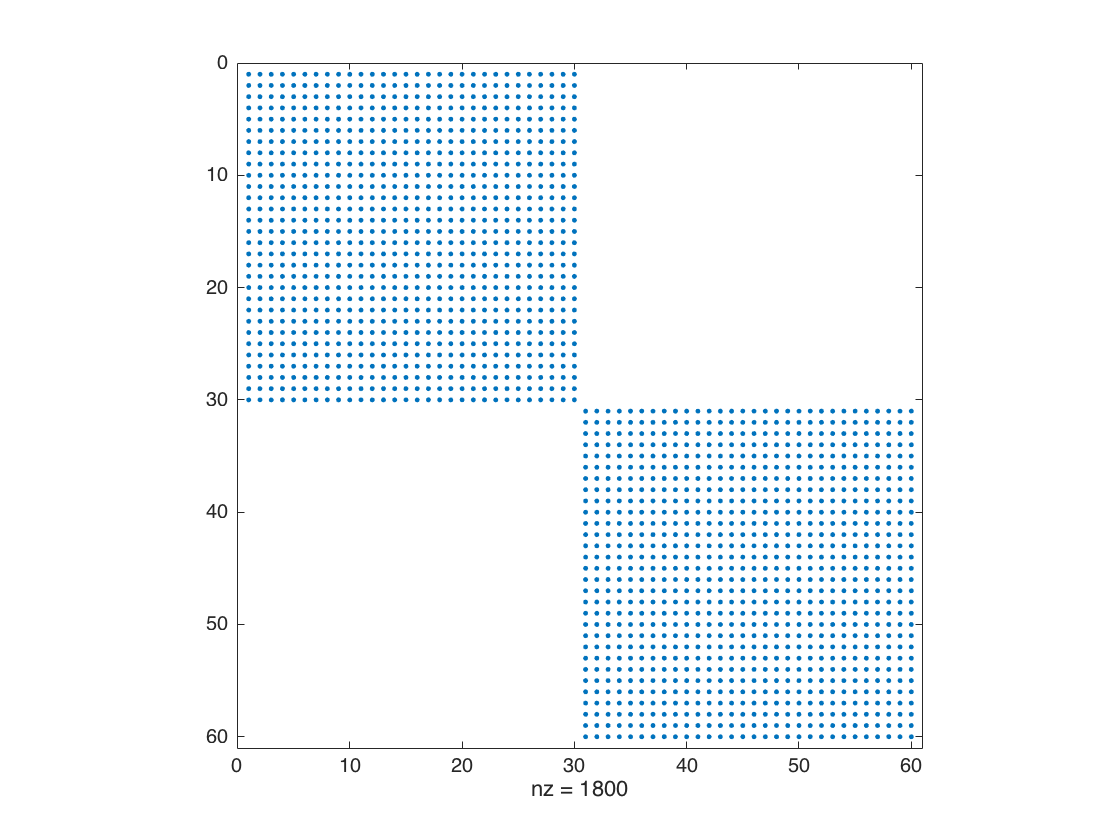
\includegraphics[width=\linewidth]{mass_spy_2p}
	\caption{Sparsity Pattern of $\vect{M^{(n-1)}}$ with $p=5$}
	\label{mass_spy}
	\endminipage
\end{figure} 
 From the mass matrix surface plot above, we further find out that the mass matrix is a diagonally dominant matrix. This is a good news for finding preconditioners for the mass matrix. Later on, a few ideas will be tried to obtain a cheap fast preconditioner.   \\
 
 \subsubsection{Jacobi Preconditioning}
 Technically speaking, Jacobi preconditioning also known as diagonal scaling, is originally a preconditioning technique used for Krylov subspace iterative solvers. Nowadays being widely used as a smoother for multigrid solvers etc.. In this case, since the mass matrix is indeed a diagonally dominant matrix, Jacobi preconditioning seems to be a simple and good preconditioner. \\  
 
 The following figure \ref{mass_precond} plots the condition number change before and after Jacobi preconditioning. 
 \begin{figure}[H]
 	\centering
 	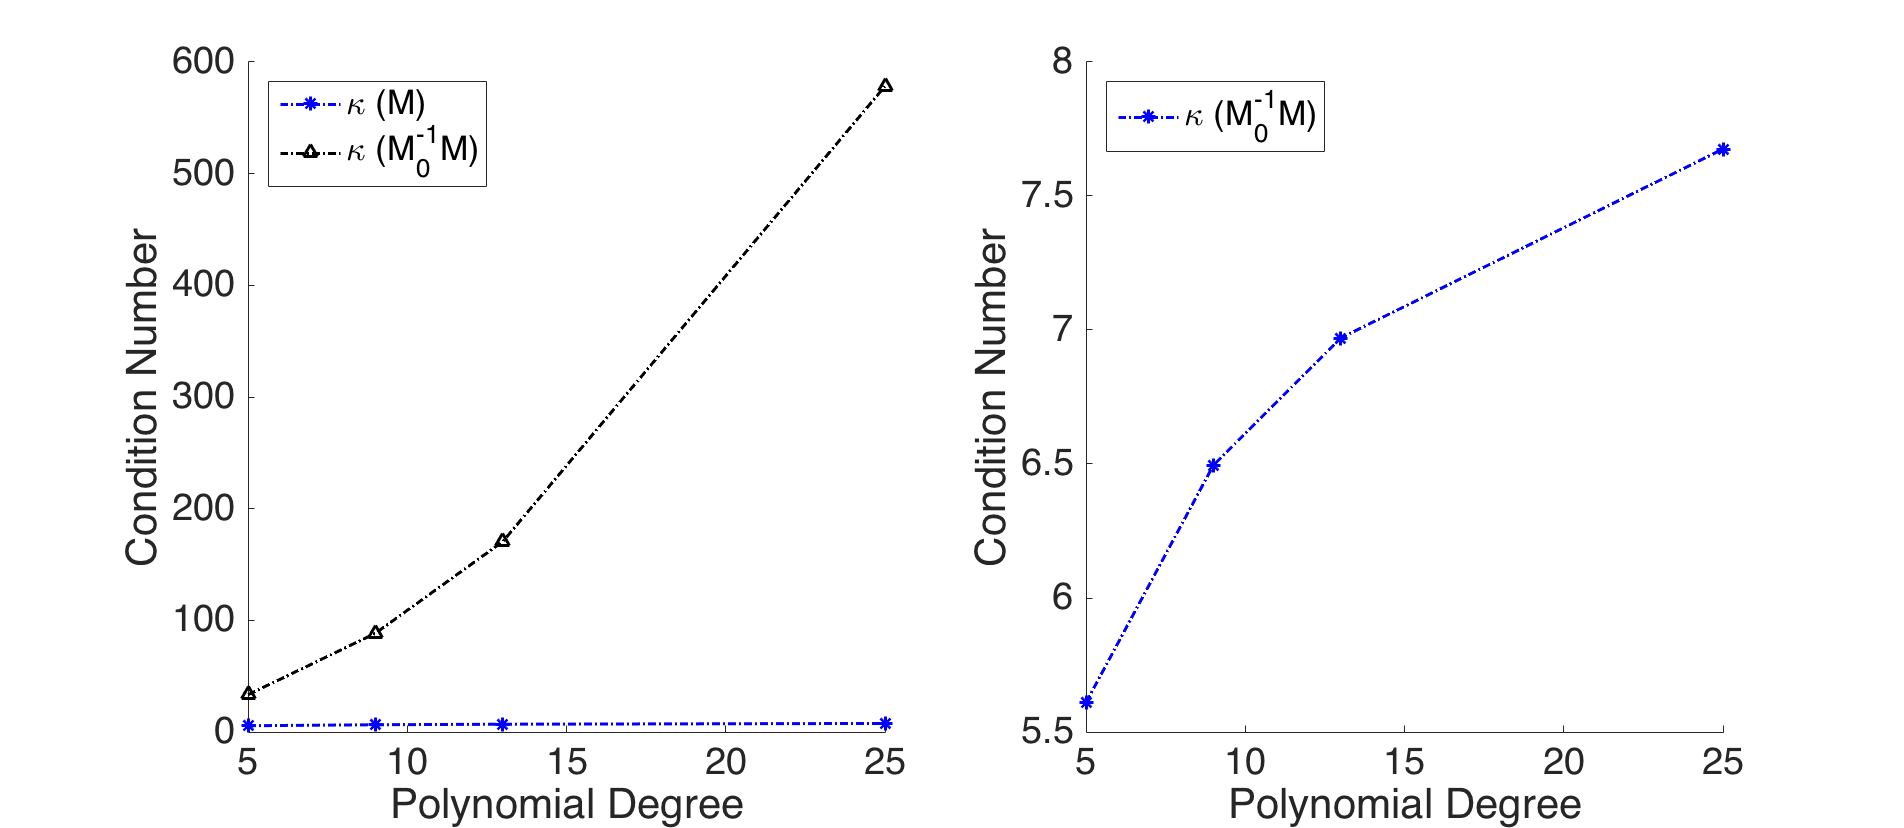
\includegraphics[width=.95\textwidth]{mass_diag_precond}
 	\caption{Condition Number of Mass Matrix Before and After Diagonal Scaling}
 	\label{mass_precond}
 \end{figure}
 We observed that the diagonal scaling suppressed the pitching-up trend of the mass matrix condition number, and significantly reduced the absolute value of the condition number. This tells us that the diagonal dominance of the mass matrix is increasing. This is an important information that leads to further improvements in making a good preconditioner. \\

If we inspect the reason of the diagonal dominance, we can see that both mass matrices of 1D basis are increasingly diagonally dominant as the expansion order increases. Because the higher the order of expansion basis goes, the closer they are to be exactly orthogonal. The next preconditioner will make use of the orthogonality of the basis. \\ 

\subsubsection{Orthogonal Basis Preconditioner}
In this section, we will make use of the unique structure of the mass matrix to construct a new preconditioner. If we take an element $m_{(K_1,K_2)}$ from the $(2,2)$ block of the mass matrix $\vect{M_v^{(n-1)}}$, we can make the following decomposition:
\begin{subequations}
	\begin{align}
		m_{(K_1,K_2)} &= \iint_{\Omega} h_p(x)e_q(y) \cdot h_m(x)e_n(y) dxdy \\
		&= \int_{x_0}^{x_{N+1}} h_p(x)h_m(x) dx  \cdot \int_{y_0}^{y_{N+1}} e_q(y)e_n(y) dy \\
		&= \lambda _{(p,m)} \cdot \mu _{(q,n)},
	\end{align}
\end{subequations}
where $\lambda_{(p,m)}$ and $\mu _{(q,n)}$ are elements from mass matrix $\vect{M_{\lambda}^{(0)}}$ produced by 1D nodal basis and mass matrix $\vect{M_{\mu}^{(1)}}$ produced by 1D edge basis functions. Thus the mass matrix of $\vect{\hat{q}^{(n-1)}}$ admits this tensor product factorisation:
\begin{equation}
	\vect{M_v^{(n-1)}} = \vect{M_{\lambda}^{(0)}} \otimes \vect{M_{\mu}^{(1)}}.
\end{equation}
The surface plot below will demonstrate this tensor product in a graphical sense. More importantly, the mass matrix eigenvalue spectra would follow the same tensor product structure! This helps us design and analyse preconditioners. We will have a little discussion on this matrix tensor product properties in the next small section. \\
  
\begin{figure}[H]
	\centering
	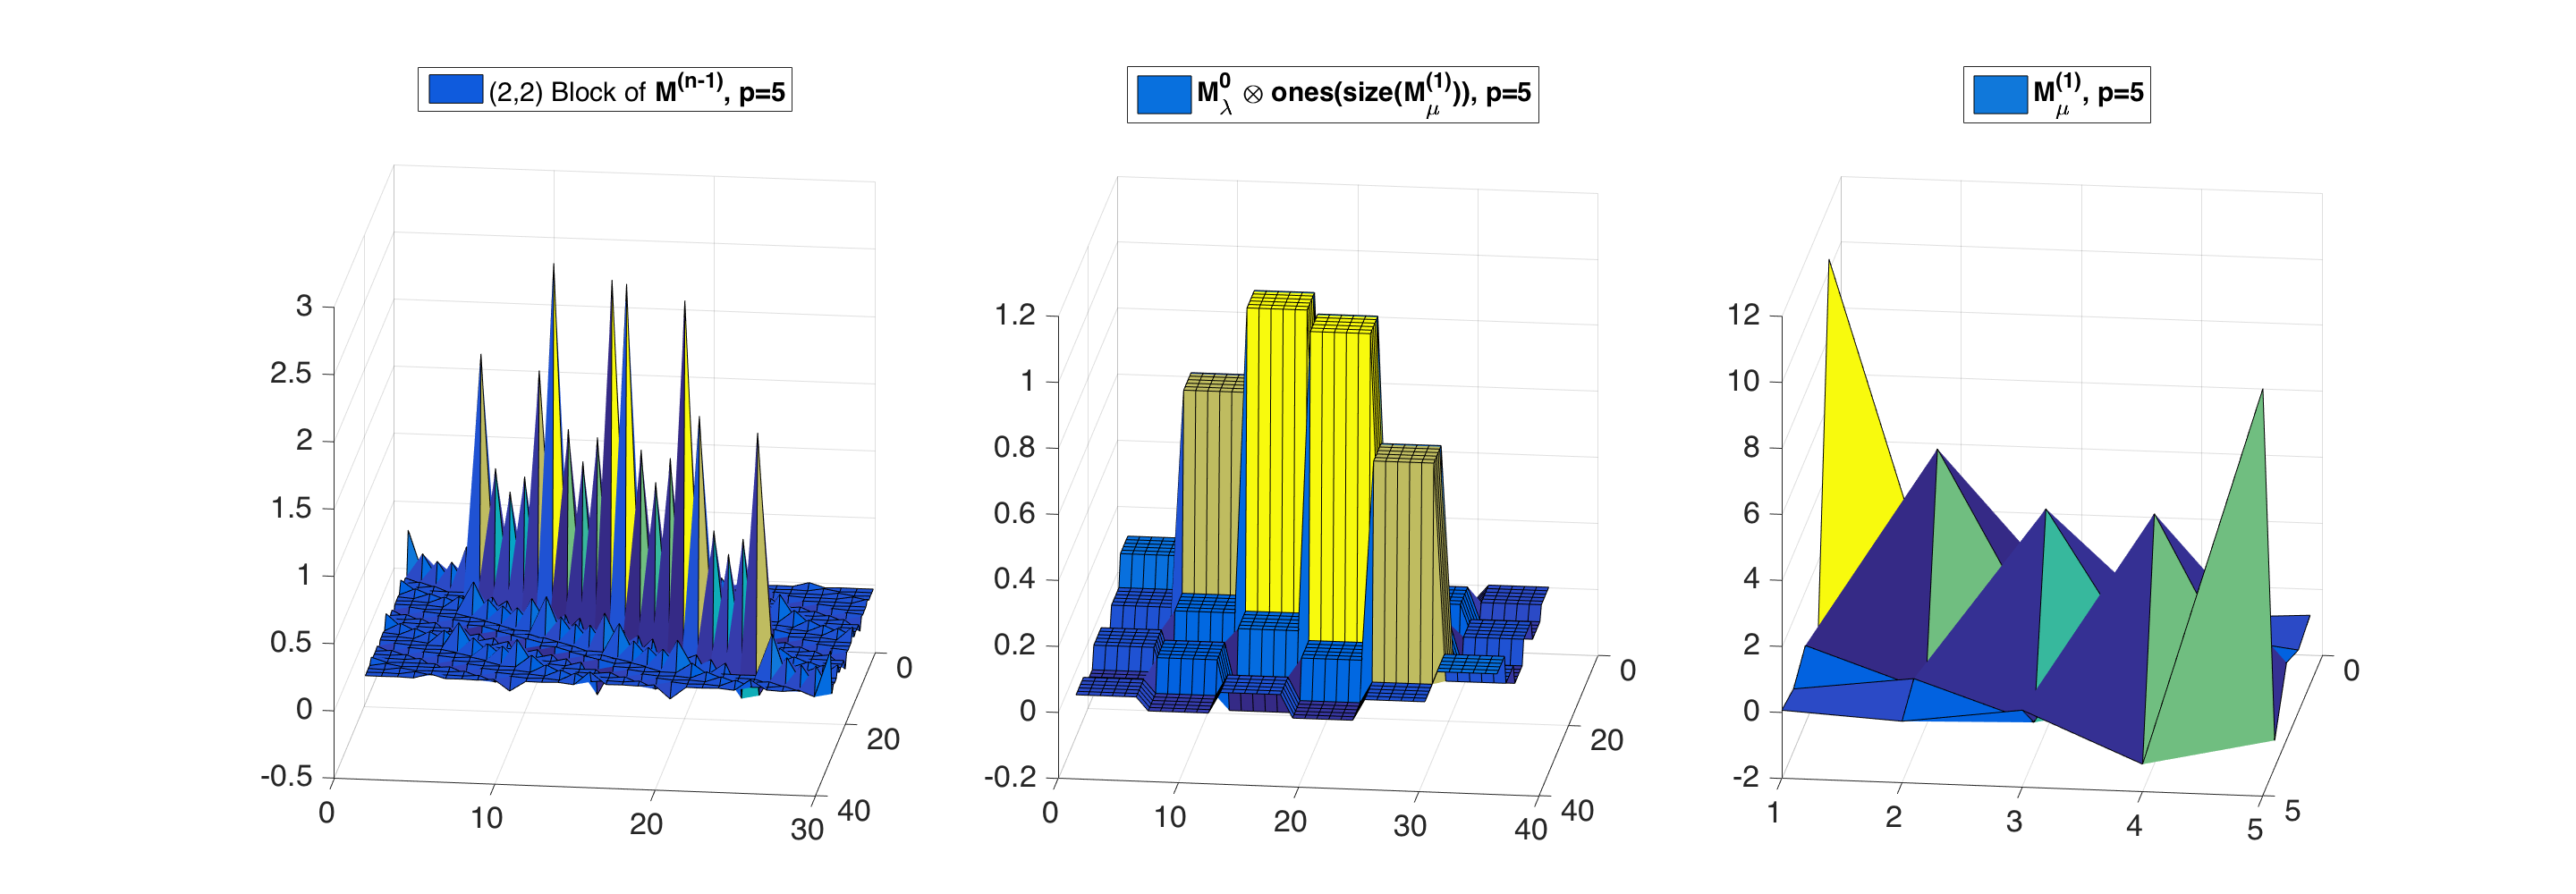
\includegraphics[width=\textwidth]{Tensor_product}
	\caption{Tensor Product Decomposition of Mass Matrix}
	\label{TensorDecompo}
\end{figure} 
It is obvious from the surface plot above that the left mass matrix is composed by the middle one for the global shape, and the right one for the local shape scaling. According to the tensor product decomposition, we can see how the numbering scheme (compression map) affects the final shape of the mass matrix. \\

Now, we use a trick to produce a preconditioner. While evaluating the integrations in mass matrix $\vect{M_{\lambda}^{(0)}}$, we use Gauss quadrature with nodal basis functions. If we specify the quadrature basis function set as exactly the same set of reduction basis functions, we would be able to obtain an orthogonal co-chain expansion vector space. In other words, $\int_{x_0}^{x_{N+1}} h_p(x)h_m(x) dx = \lambda _{(p,m)}\cdot \delta_{pm}$, $\delta$ is the Kronecker delta. This trick made $\vect{M_{\lambda}^{(0)}}$ a diagonal matrix if the basis function follows the numbering scheme as in figure \ref{num_scheme}. Thus the final mass matrix $\vect{M_0^{(n-1)}}$ will have a very fine block diagonal structure. 
\begin{figure}[H]
	\centering
	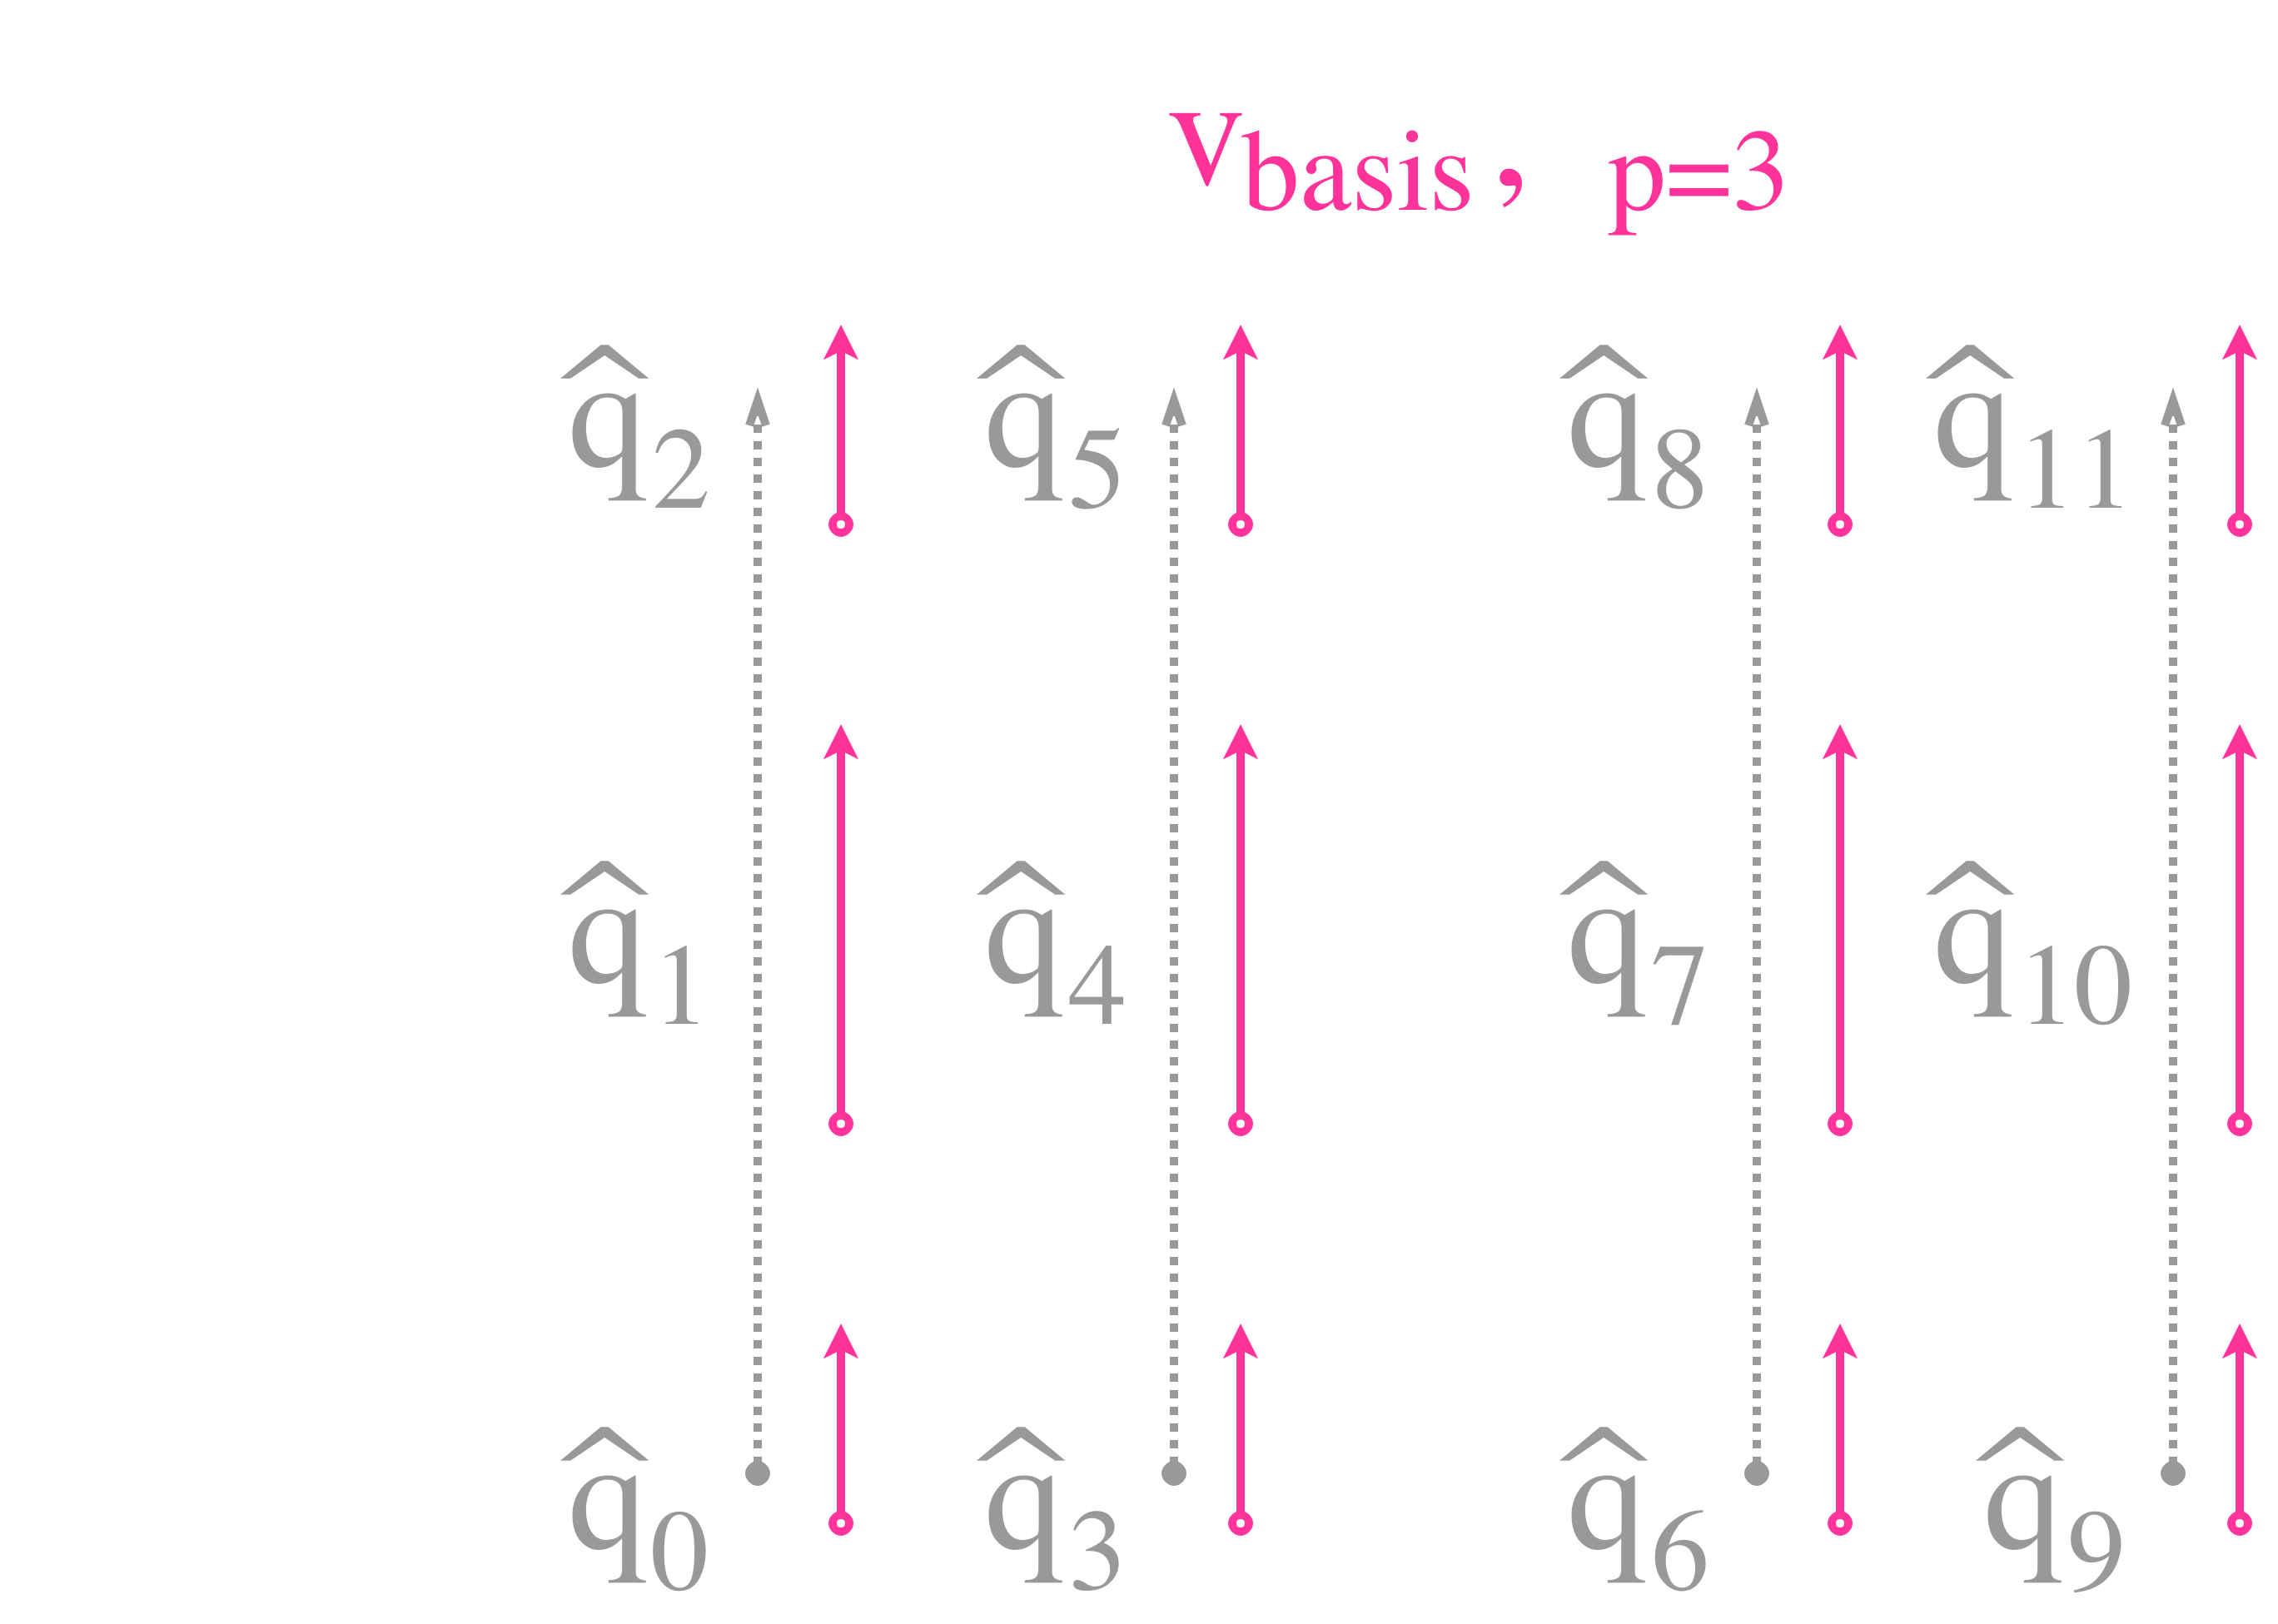
\includegraphics[width=.4\textwidth]{num_scheme}
	\caption{Numbering Scheme of Basis Functions}
	\label{num_scheme}
\end{figure} 
The block diagonal mass matrix will be shown below:
\begin{figure}[H]
	\minipage{0.45\textwidth}
	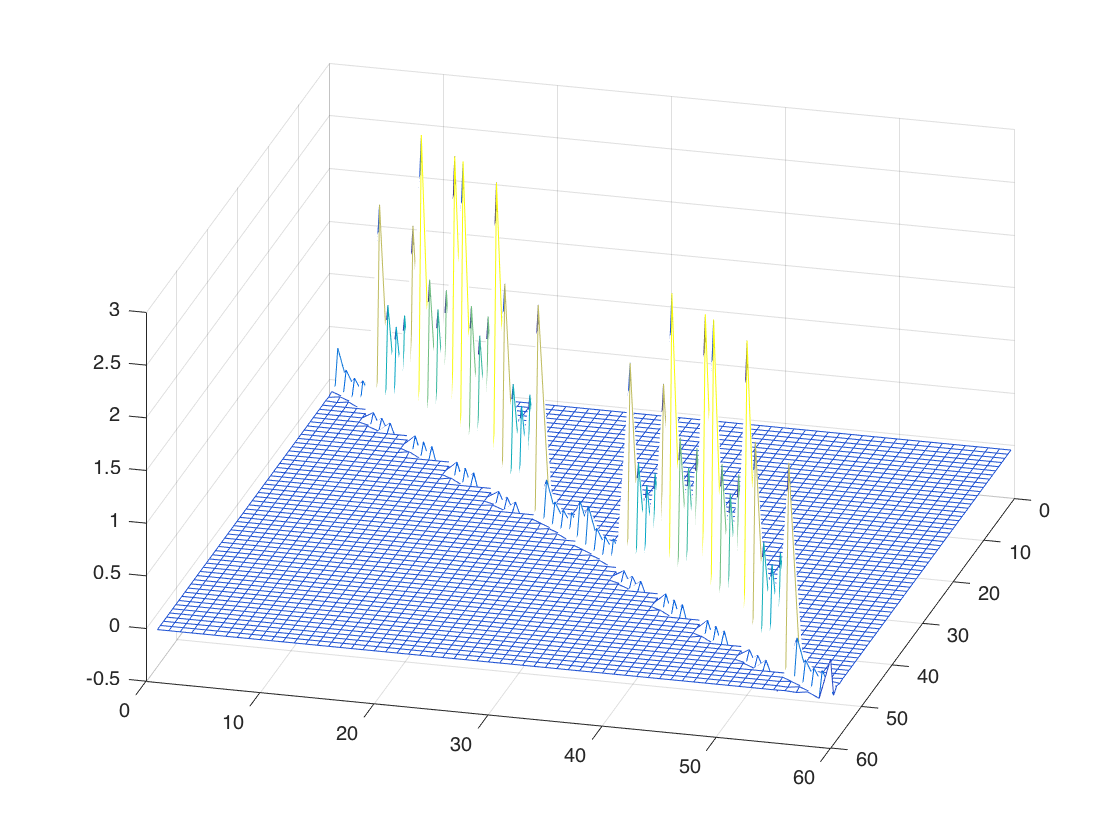
\includegraphics[width=\linewidth]{full_mass_quad_1p}
	\caption{$\vect{M_0^{(n-1)}}$ with $p=5$}
	\label{mass_surf}
	\endminipage \hfill
	\minipage{0.45\textwidth}
	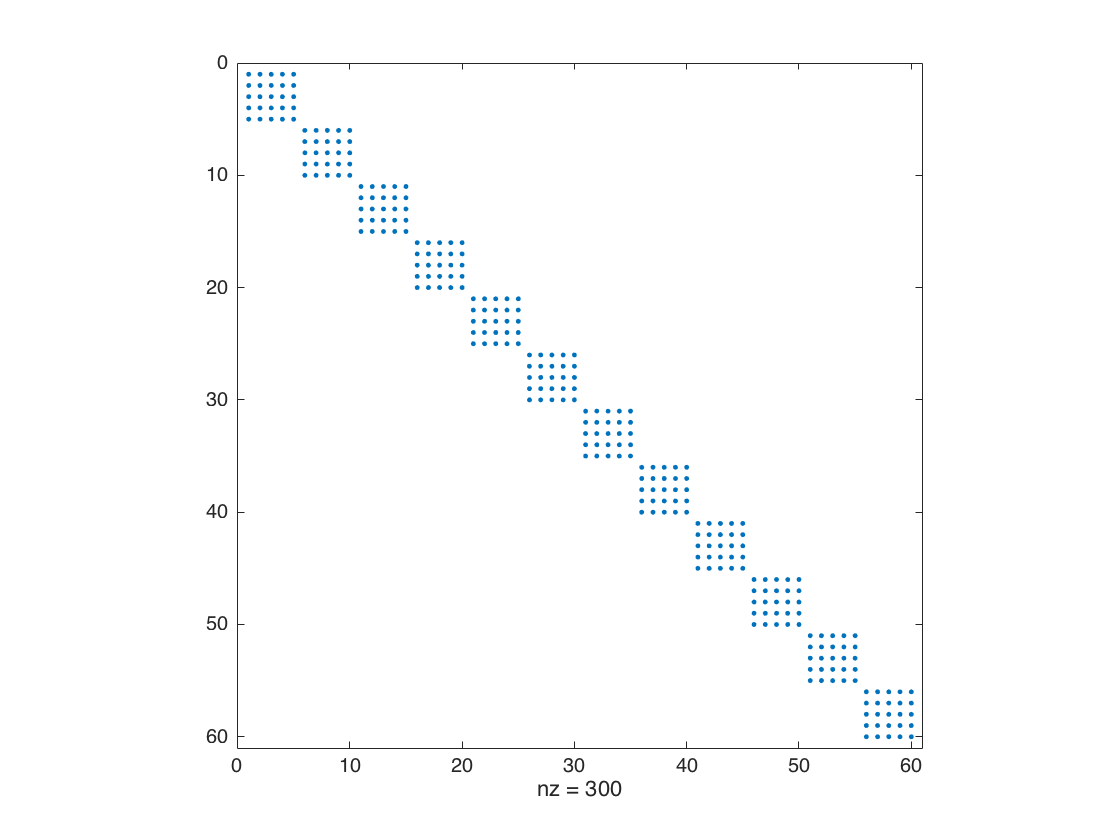
\includegraphics[width=\linewidth]{mass_spy_1p}
	\caption{Sparsity Pattern of $\vect{M_0^{(n-1)}}$ with $p=5$}
	\label{mass_spy}
	\endminipage
\end{figure}
Within each block, the shape would be exactly the same as the mass matrix $\vect{M_{\mu}^{(1)}}$. The new preconditioner is easily and fast invertible, and also easy in storage and manipulation, because $\vect{M_v^{(n-1)^{-1}}} = \vect{M_{\lambda}^{(0)^{-1}}} \otimes \vect{M_{\mu}^{(1)^{-1}}}$. In this case $\vect{M_{\lambda}^{(0)^{-1}}}$ is a diagonal matrix, thus the work load of taking the inverse only scales with the mass matrix size $\vect{M_{\mu}^{(1)^{-1}}}$. \\

Now, we will show the performance of this preconditioner in figure \ref{orth_precond}.
\begin{figure}[H]
	\centering
	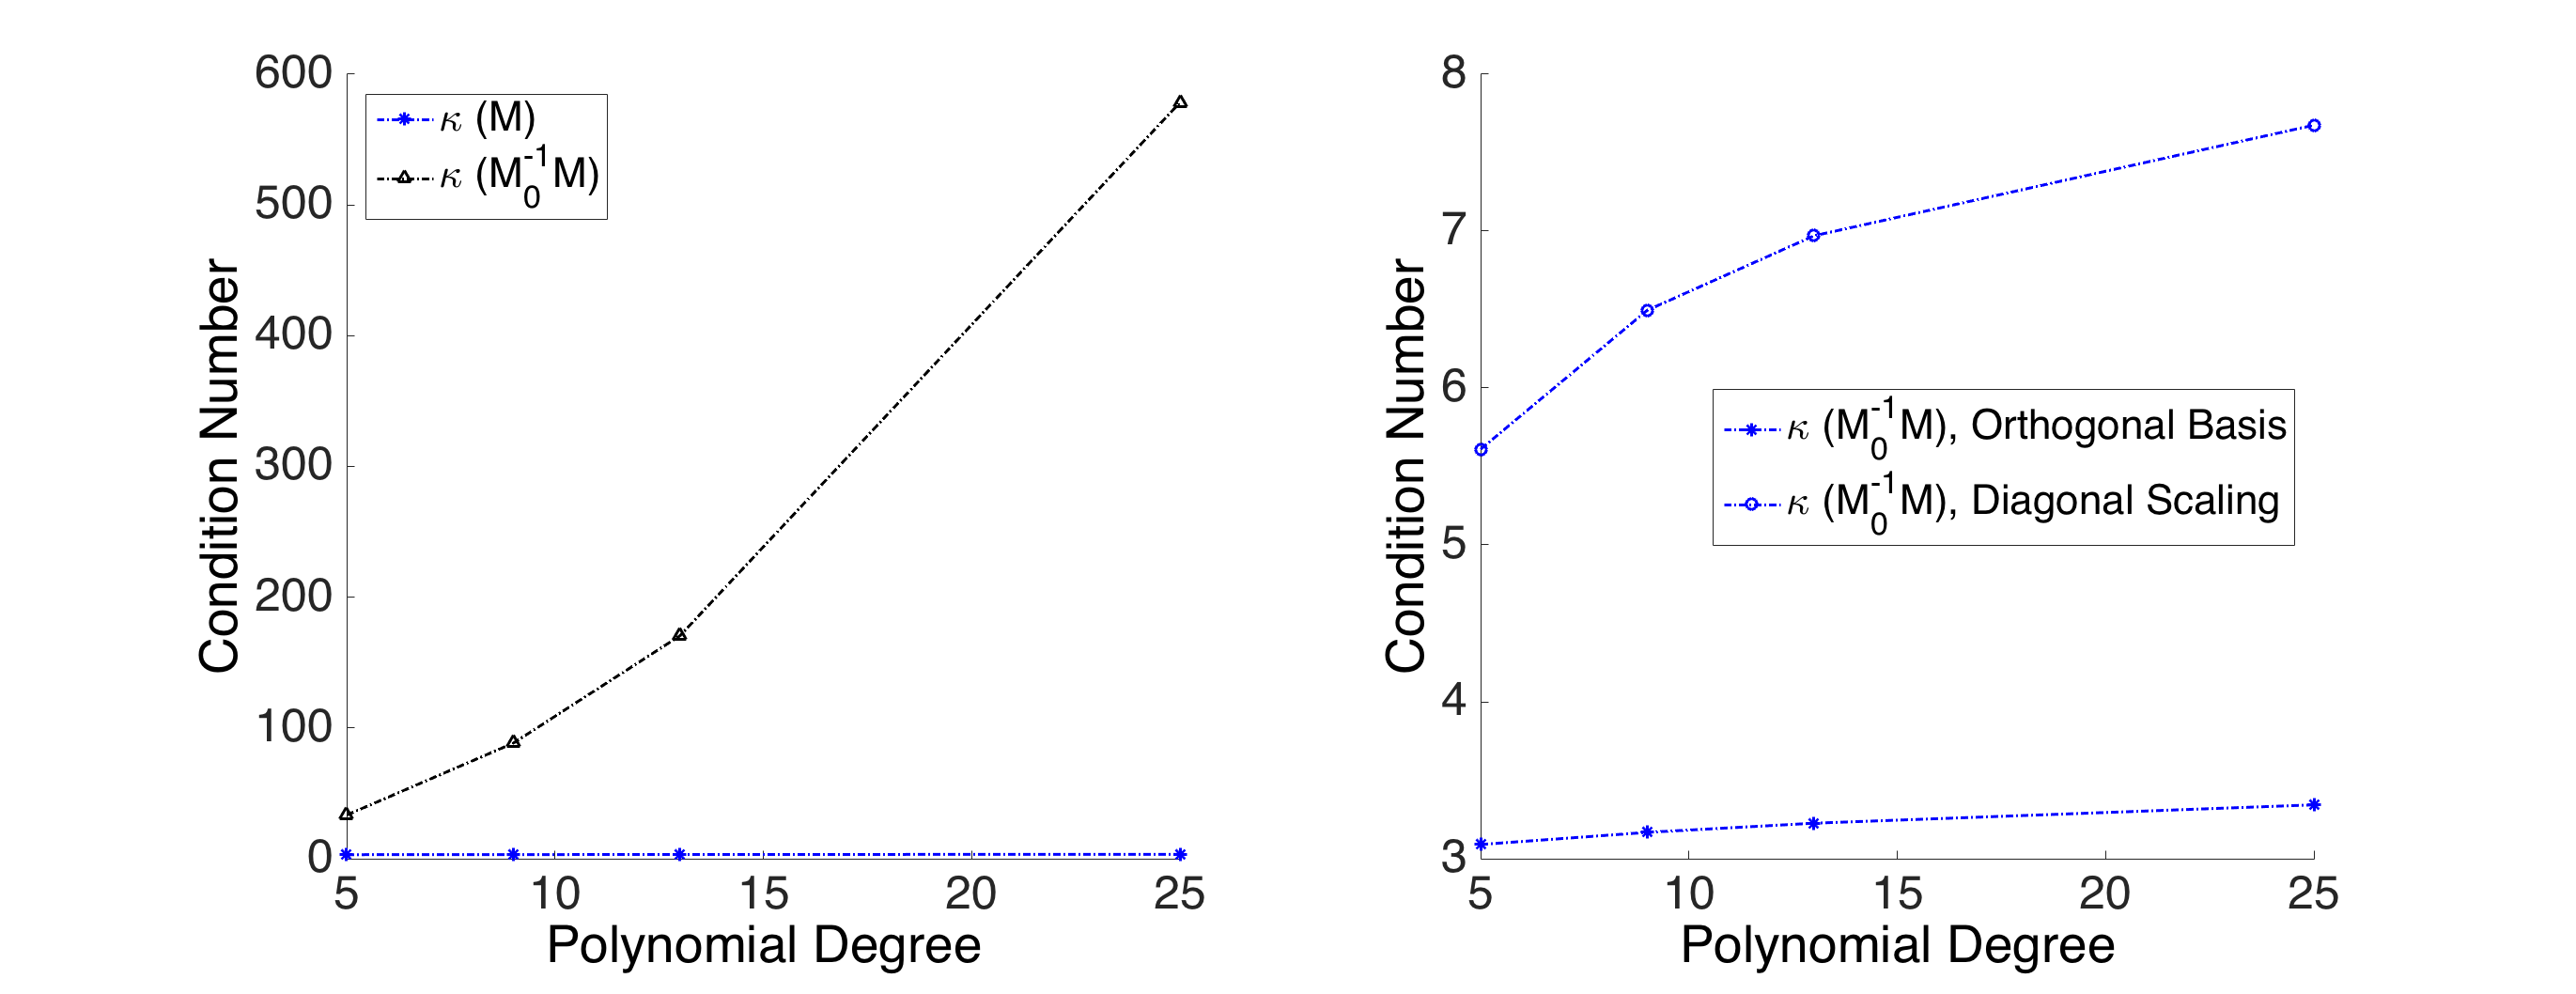
\includegraphics[width=.95\textwidth]{mass_orth_precond}
	\caption{Performance of Orthogonal Basis Preconditioner}
	\label{orth_precond}
\end{figure}
From the figure above, we surely see that the performance of the Orthogonal Basis preconditioner is much more stable and produce a preconditioned mass matrix whose conditioner number is nearly independent from the problem size. \\

\subsection{Discussion on Matrix Kronecker Product}
This is an additional discussion on the properties of the matrix Kronecker product. They could reveal the block structure of matrices and could be very helpful in analysing the spectral property, sparsity pattern, and matrix ordering (numbering), etc., especially for PDE induced linear equation systems. \\

We introduce two matrices: $\vect{A_{pm\times qn}} = \vect{{A_1}_{p\times q}} \otimes \vect{{A_2}_{m\times n}}$ and $\vect{B_{qn\times ro}} = \vect{{B_1}_{q\times r}} \otimes \vect{{B_2}_{n\times o}}$. We will use them in the coming discussion. \\

\subsubsection{Permutation of Kronecker Product}
Tensor product is not permutable. But there exists a pair of unique permutation matrices $(\vect{P_{pm\times pm}},\vect{Q_{qn\times qn}})$ that helps the permutation: 
\begin{equation}
	\vect{P_{pm\times pm}}\left( \vect{{A_1}_{p\times q}} \otimes \vect{{A_2}_{m\times n}}\right) \vect{Q_{qn\times qn}} = \vect{{A_2}_{m\times n}} \otimes  \vect{{A_1}_{p\times q}}.
\end{equation} 
Moreover, when $p=q$ and $m=n$, $\vect{P} = \vect{Q^T}$. \\

Using this property, we understand how the numbering scheme change the ordering of the mass matrix:
\begin{equation}
	\vect{P}\left( \vect{M^{(0)}_{\lambda}} \otimes \vect{M^{(1)}_{\mu}}\right) \vect{P^T} = \vect{M^{(1)}_{\mu}} \otimes \vect{M^{(0)}_{\lambda}}.
\end{equation}
This tells us that the sparsity pattern of mass matrix is affected by the numbering scheme while the spectrum is not.\\

\subsubsection{Mixed Product Property}
The Kronecker product could be mixed with matrix product:
\begin{equation}
	\vect{A_{pm\times qn}} \vect{B_{qn\times ro}} = \left(\vect{{A_1}_{p\times q}} \vect{{B_1}_{q\times r}} \right) \otimes \left( \vect{{A_2}_{m\times n}}\vect{{B_2}_{n\times o}} \right).
\end{equation}
Thus, if the mass matrices admits diagonalisations: 
\begin{subequations}
\begin{align}
	\vect{M_v^{(n-1)}} &= \vect{T \Lambda T^T}, \\
	\vect{M_{\lambda}^{(0)}} &= \vect{T_\lambda \Lambda_\lambda T_\lambda^T},\\
	\vect{M_{\mu}^{(1)}} &= \vect{T_\mu \Lambda_\mu T_\mu^T},
\end{align}
\end{subequations}
then we have:
\begin{equation}
\begin{split}
	\vect{M_v^{(n-1)}} &= \vect{M_{\lambda}^{(0)}} \otimes \vect{M_{\mu}^{(1)}}\\
	&= \left(\vect{T_\lambda} \otimes	\vect{T_\mu} \right)\left(\vect{\Lambda_\lambda} \otimes \vect{\Lambda_\mu} \right) \left(\vect{T_\lambda^T} \otimes \vect{T_\mu^T} \right) \\
	&= \vect{T \Lambda T^T}.
\end{split}
\end{equation}
This tells us that the spectrum of the big mass matrix is spanned by small mass matrices. What's more, many symmetric iterative solvers require symmetric preconditioners which need to compute the Cholesky factorisation of the mass matrix. With this Kronecker product, the calculation load no longer scales with the 2D problem size, but with two 1D problem size. For direct solvers, the preconditioner is the inverse of mass matrix, which could also be calculated by inverting the small mass matrices. \\

About this matrix tensor product, we give one more example of how it helps us understand the block structure of the coefficient matrices. Take the Schur complement of the mass matrix:
\begin{equation}
	\vect{S} = \vect{W^T E M^{-1} E^T W} = \vect{W^T G W}.
\end{equation}      
The incidence matrix has a block structure: 
\begin{equation}
	\vect{E} = \begin{bmatrix}
		\vect{D_u} & \vect{D_v} 
	\end{bmatrix},
\end{equation}
corresponding to the block diagonal structure of the mass matrix:
\begin{equation}
	\vect{M} = \begin{bmatrix}
		\vect{M_u} & \vect{O} \\
		\vect{O} & \vect{M_v}
	\end{bmatrix}.
\end{equation}
Thus we have: 
\begin{equation}
	\vect{G} = \vect{E M^{-1} E^T} = \vect{D_u {M_u}^{-1} {D_u}^T} + \vect{D_v {M_v}^{-1} {D_v}^T} .
\end{equation}
Further more, we have:
\begin{equation}\label{eqn:Schur}
\begin{split}
	\vect{D_v {M_v}^{-1} {D_v}^T}  &= \left(\vect{D \otimes I} \right)\left(\vect{M_{\lambda}^{(0)}} \otimes \vect{M_{\mu}^{(1)}} \right) \left(\vect{D^T \otimes I^T} \right) \\
	&= \left(\vect{D M_{\lambda}^{(0)} D^T} \right) \otimes \vect{M_{\mu}^{(1)}}
\end{split}
\end{equation}
where $D$ is the 1D mesh incidence matrix (discrete gradient operator) and $I$ is the identity matrix. It's easy to see how the factor matrices contribute to the distorted spectrum. \\  

\subsection{Schur Complement Approximation}   
The Schur complement of the mass matrix is the most difficult part of the work, where many solution method such as the two stage Uzawa Algorithm and its variations all break down. The Schur complement matrix usually involves mapping that changes vector space dimension and has a distorted spectrum. Uzawa algorithm is introduced while solving nonlinear programming problems, and one can see that the resulted Schur complement matrix has indeed a "nonlinearly" growing condition number. Thus preconditioning is crucial for such schemes to succeed.  \\  

From the previous inspection in figure \ref{cond}, we noticed that the wedge product matrix $\vect{W}$ barely contribute to the growth of $\kappa(\vect{S})$. Thus we ignore the wedge product matrix while constructing the preconditioner. This leads to a preconditioner $\vect{G_0} = \vect{E M_0^{-1} E^T}$ that approximates the Schur complement matrix. \\

If we continue the analysis in equation \ref{eqn:Schur}, we notice that with symmetric numbering scheme, $\vect{M_u} = \vect{M_v}$, $\vect{D_u}$ and $\vect{D_v}$ are connected by row permutation $\vect{P}$:
\begin{equation}
	\vect{PD_u} = \vect{D_v}.
\end{equation} 
Thus,
\begin{equation}
	\vect{G} = \vect{P (D_v {M_v}^{-1} {D_v}^T )P^T}  + \vect{D_v {M_v}^{-1} {D_v}^T} .
\end{equation}
Further more, due to the symmetry of the co-ordinate system, it has to be the case that: $\vect{P} = \vect{P^T}$. \\

\subsubsection{First Attempt}
The first attempt of finding a preconditioner for $\vect{S}$ is done by following a conventional simplification in many literatures, which is to replace mass matrix with an identity matrix. We get $\vect{G_0} = \vect{map} = \vect{E\cdot E^T}$, the finite difference Laplacian of a uniform mesh. This first attempt reveals the sparsity pattern of the preconditioner and shows how effective this preconditioner configuration could be. The sparsity pattern of $\vect{G_0}$ is given in figure \ref{spylaplacian}.
\begin{figure}
	\minipage{0.45\textwidth}
	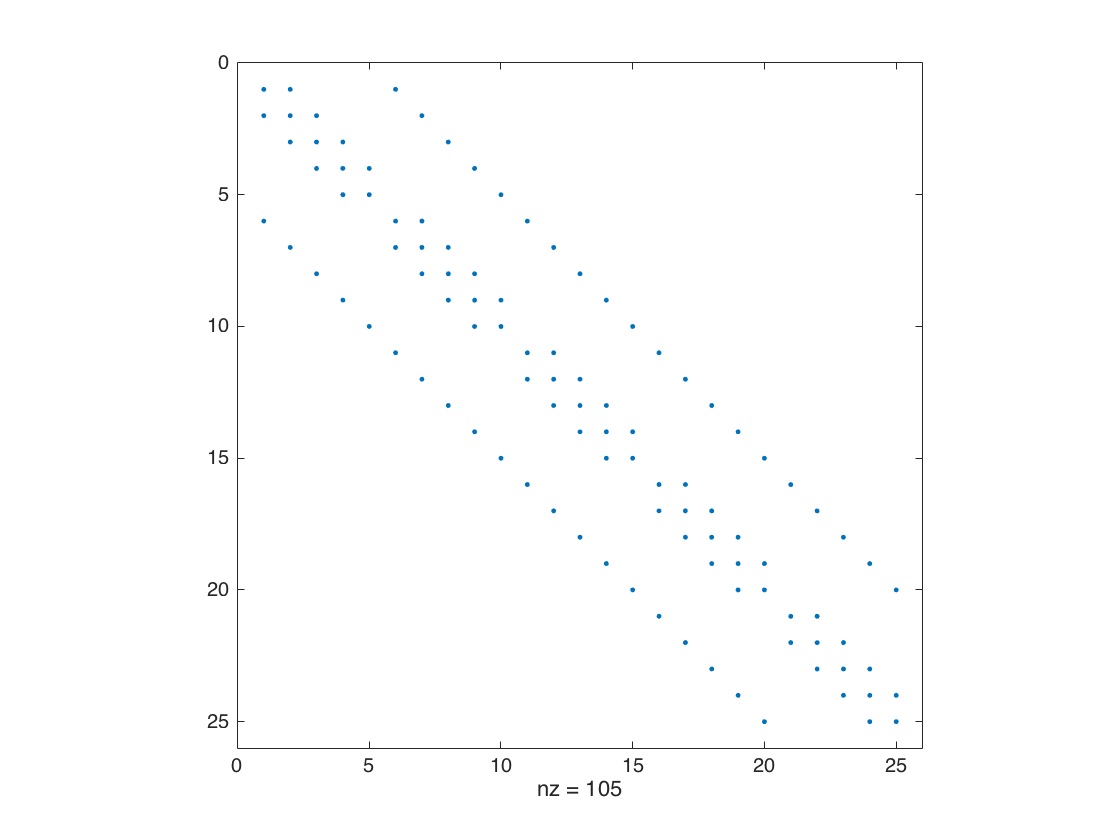
\includegraphics[width=\linewidth]{spy_map}
	\caption{Finite Difference Laplacian Sparsity Pattern}
	\label{spylaplacian}
	\endminipage \hfill
	\minipage{0.45\textwidth}
	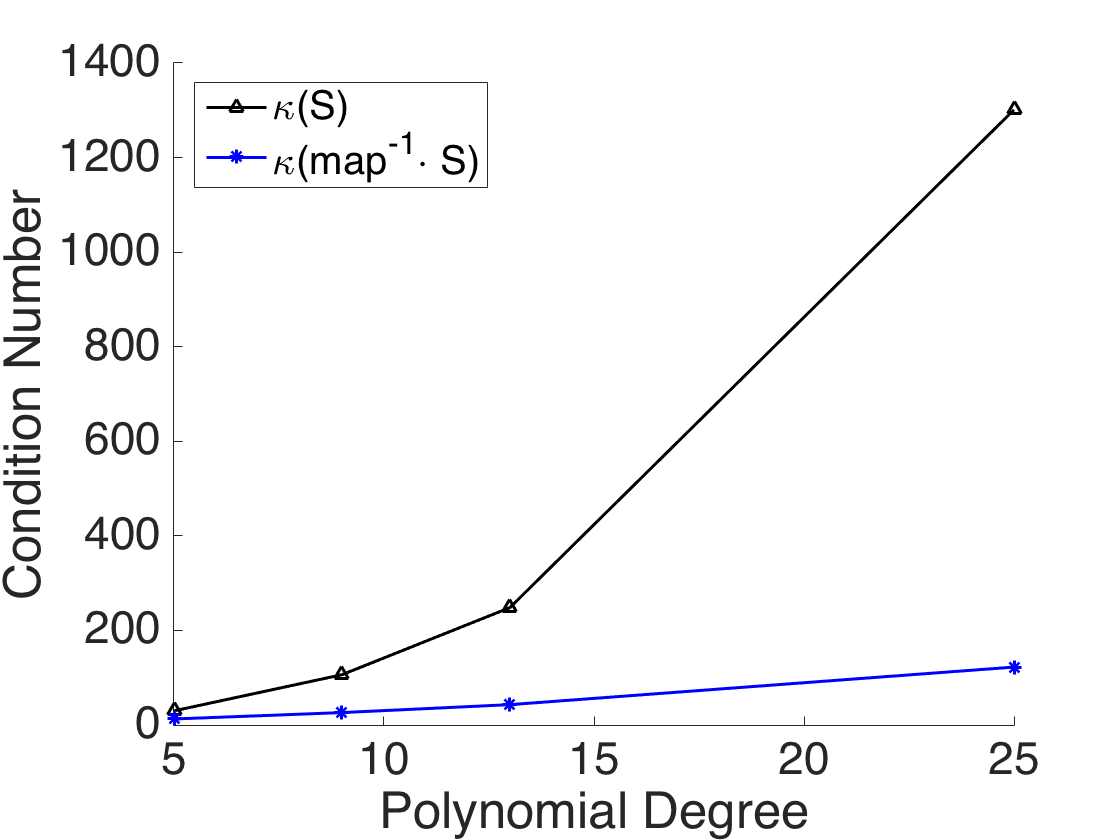
\includegraphics[width=\linewidth]{firstattempt}
	\caption{Condition Number Before and After Preconditioning}
	\label{firstatt}
	\endminipage 
\end{figure}
We know that $\vect{G_0} = \vect{P (D_v {D_v}^T )P^T}  + \vect{D_v {D_v}^T}$, and the mapping $f(\vect{\cdot}) = \vect{P[\cdot]P^T}$ won't change the diagonal dominance of any diagonal dominant matrix . Thus we hope that $\vect{D_v {M}^{-1} {D_v}^T}$ in the preconditioner is diagonal dominant and has a very thin diagonal bandwidth. If we apply the mass matrix approximates developed in the previous section to obtain approximate of $\vect{G}$, the best sparsity we can get will be no better as in figure \ref{spylaplacian}. Now we want to know if $\vect{G_0}$ could really improve the Schur complement matrices condition, thus we present the outcome of the first attempt in figure \ref{firstatt}. \\

\subsubsection{Schur Complement Approximate}
In this section, we will use mass matrix approximates developed before to construct preconditioners for the Schur complement. First we will use the Jacobi preconditioner to compute $\vect{G_1} = \vect{E {M_{Jacob}}^{-1} {E}^T}$. Since $\vect{M_0}$ in this case is a diagonal matrix, the sparsity is at the best condition. Then, we compute $\vect{G_2}$ with orthogonal basis preconditioner $M_{orth}$ and make comparisons between the preconditioners we have had by now. The results are shown in the following figure \ref{schur_pre}.
\begin{figure}[H]
	\centering
	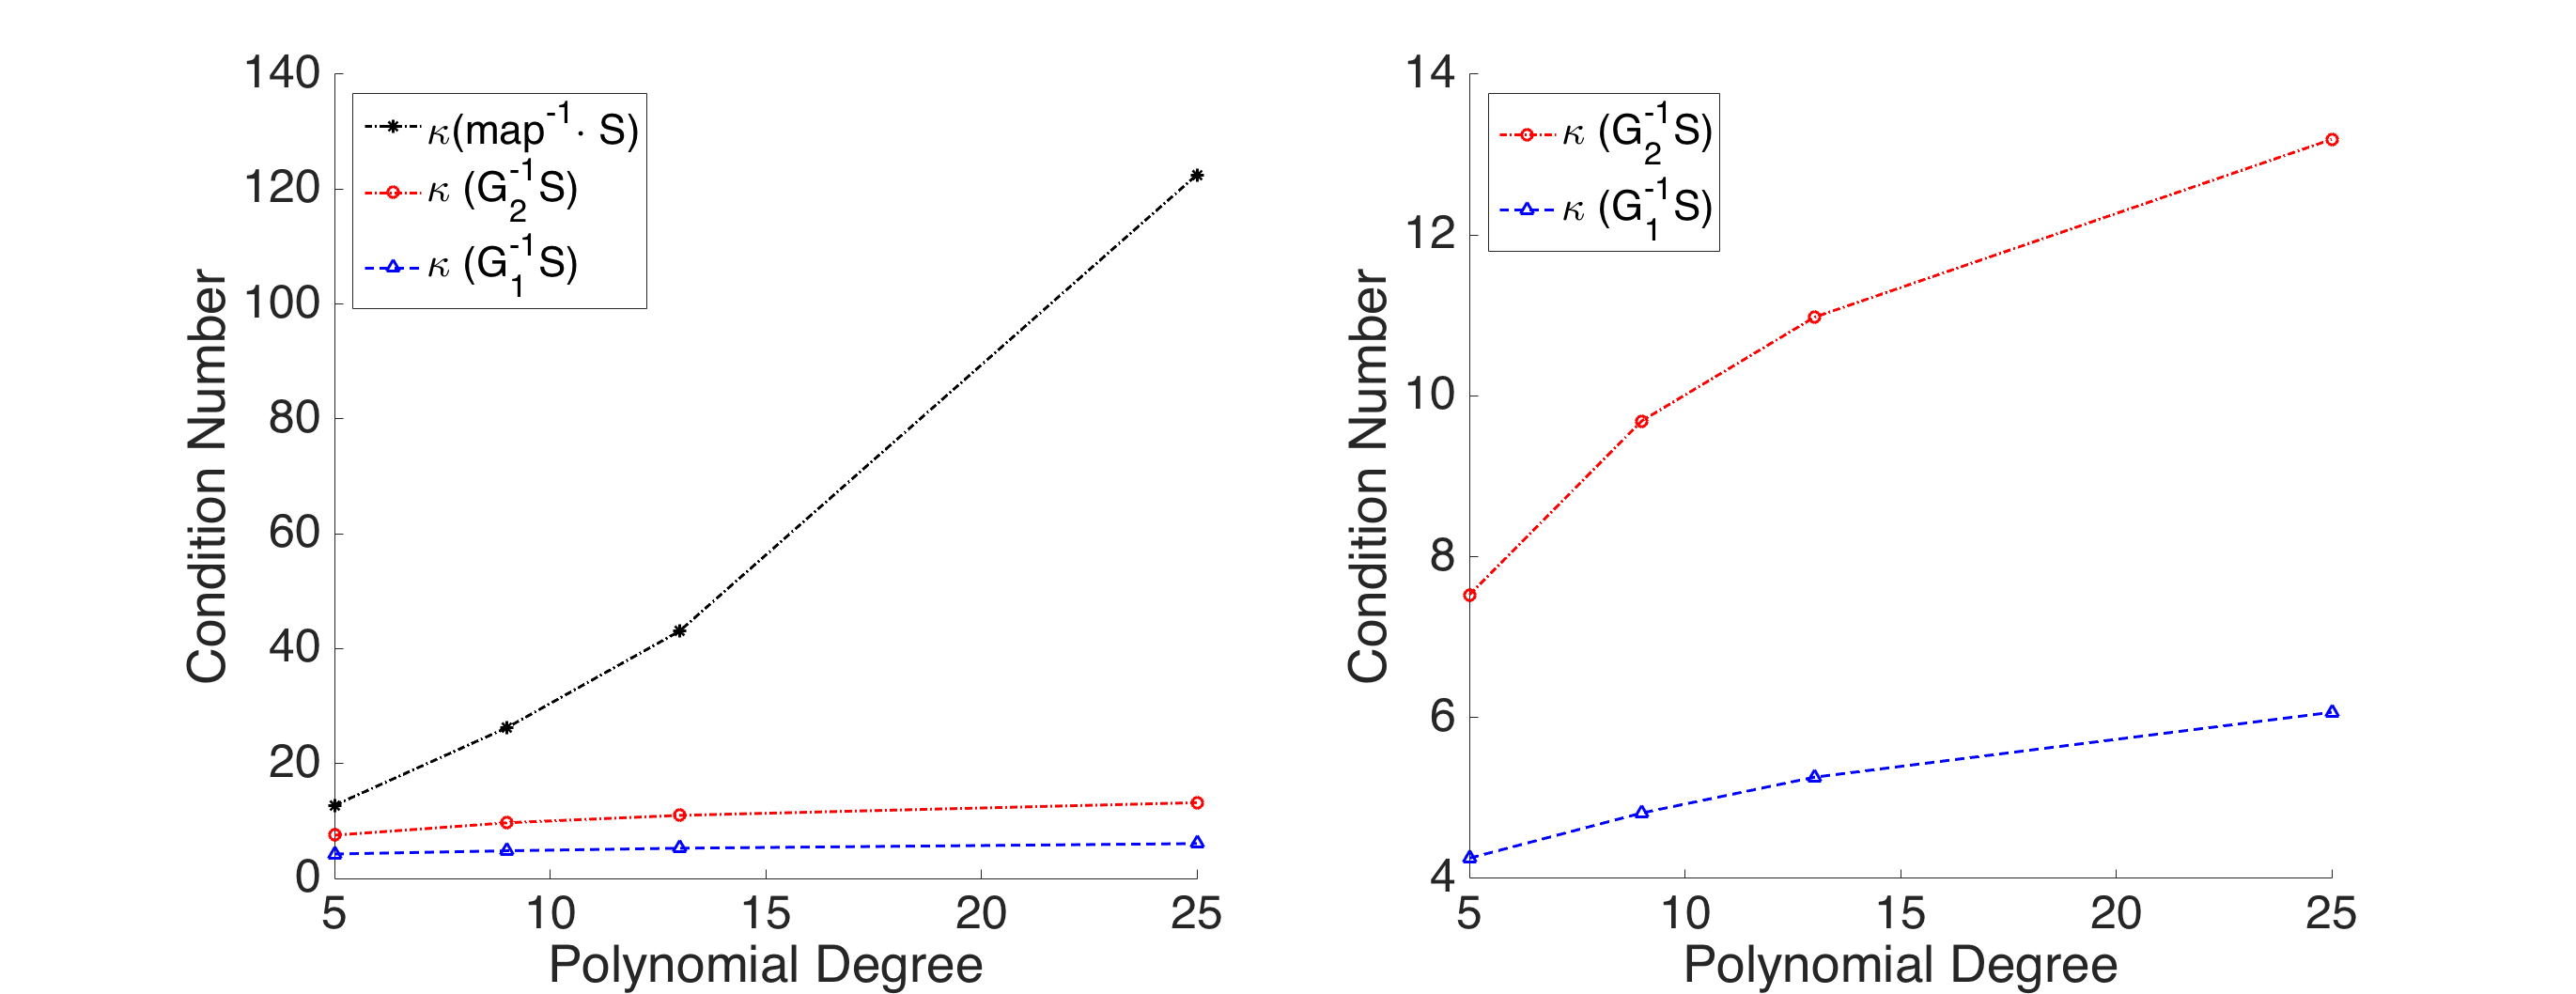
\includegraphics[width =.95\textwidth]{Schur_precond}
	\caption{Condition Number After Preconditioning}
	\label{schur_pre}
\end{figure}
Surprisingly, the diagonal scaling is the best preconditioner for the Schur complement. This is probably because we dropped the wedge product matrix while constructing the preconditioner. 
            








    

 
 
 
 
 
 
 
 
 
  
 


   
        










  